% This is Information Sciences and Technologies Bulletin of the ACM Slovakia template
% based on:
% THIS IS SIGPROC-SP.TEX - VERSION 3.1
% WORKS WITH V3.2SP OF ACM_PROC_ARTICLE-SP.CLS
% APRIL 2009
%
% It is an example file showing how to use the 'acmbulletin.cls' V3.2SP
% LaTeX2e document class file for Conference Proceedings submissions.
% ----------------------------------------------------------------------------------------------------------------
% This .tex file (and associated .cls V3.2SP) *DOES NOT* produce:
%        Page numbering
% ---------------------------------------------------------------------------------------------------------------
% It is an example which *does* use the .bib file (from which the .bbl file
% is produced).
% REMEMBER HOWEVER: After having produced the .bbl file,
% and prior to final submission,
% you need to 'insert'  your .bbl file into your source .tex file so as to provide
% ONE 'self-contained' source file.
%
% Questions/suggestions regarding the guidelines, .tex and .cls files, etc. to
% lacko@fiit.stuba.sk
%
% For tracking purposes - this is V3.1SP - APRIL 2009

\documentclass{acmbulletin}

	\usepackage[papersize={210mm,297mm}, top=0cm]{geometry}
	\topmargin -2cm
	\headheight 1cm
	\headsep 1cm
	\oddsidemargin -0.5cm
	\evensidemargin -0.5cm
	\textwidth 17.0cm
	\textheight 25.0cm
	\usepackage{fancyhdr}
	\pagestyle{fancy}
	\fancyhf{}

	\usepackage[slovak,english]{babel}
	\usepackage[T1]{fontenc}
	\usepackage[utf8]{inputenc}
	\usepackage{amsmath}
	\usepackage{amssymb,amsfonts,amscd}
	\usepackage{array,hhline}
	\usepackage{makeidx}
	\usepackage{fancyhdr}
	\usepackage{graphicx}
	\usepackage{listings}
	\usepackage{url,mathptmx}

\startpage{1}
\begin{document}
\thispagestyle{empty}

\fancyhead[LO,RE]{}
\fancyhead[CO]{Information Sciences and Technologies Bulletin of the ACM Slovakia}
\fancyhead[RO]{\thepage}
\fancyhead[CE]{Chovanec, M.: Q-function aproximation in  Q-learning algortihms using neural network}
\fancyhead[LE]{\thepage}
\title{Q-function aproximation in  Q-learning algortihms using neural network}
%
% You need the command \numberofauthors to handle the 'placement
% and alignment' of the authors beneath the title.
%
% For aesthetic reasons, we recommend 'three authors at a time'
% i.e. three 'name/affiliation blocks' be placed beneath the title.
%
% NOTE: You are NOT restricted in how many 'rows' of
% "name/affiliations" may appear. We just ask that you restrict
% the number of 'columns' to three.
%
% Because of the available 'opening page real-estate'
% we ask you to refrain from putting more than six authors
% (two rows with three columns) beneath the article title.
% More than six makes the first-page appear very cluttered indeed.
%
% Use the \alignauthor commands to handle the names
% and affiliations for an 'aesthetic maximum' of six authors.
% Add names, affiliations, addresses for
% the seventh etc. author(s) as the argument for the
% \additionalauthors command.
% These 'additional authors' will be output/set for you
% without further effort on your part as the last section in
% the body of your article BEFORE References or any Appendices.

\numberofauthors{1}
\author{
% You can go ahead and credit any number of authors here,
% e.g. one 'row of three' or two rows (consisting of one row of three
% and a second row of one, two or three).
%
% The command \alignauthor (no curly braces needed) should
% precede each author name, affiliation/snail-mail address and
% e-mail address. Additionally, tag each line of
% affiliation/address with \affaddr, and tag the
% e-mail address with \email.
%
% 1st. author
\alignauthor
Ing.\ Michal Chovanec\titlenote{
Recommended by thesis supervisor: Prof.\ Ing. \ Juraj Miček, PhD.\\
Defended at Faculty of Management of science and Informatics, University of Zilina}\\
			 \affaddr{Department of technical cybernetics}\\
       \affaddr{Faculty of Management of science and Informatics}\\
       \affaddr{Prof.\ Ing. \ Juraj Miček, PhD.}\\
       \email{michal.chovanec@yandex.com}
}

\toappear{\copyrighttext}

\maketitle
\begin{abstract}

This paper is focused on results in Q-learning value function approximation
using basis function neural network. For large state space is function
approximation necessary, but common feed forward neural network can't be learned.
We present neural network of basis functions, which can be learned using
backpropagation.

\end{abstract}

%A category with the (minimum) three required fields
\category{H.4}{Machine learning}{Artificial inteligence}
\category{H.4}{Machine learning}{Reinforcement learning}
\category{H.4}{Machine learning}{Neural networks}

\keywords{Q-learning, reinforcement learning, neural network}

\section{Introduction}

In learning systems based on supervised learning - set of inputs and
required outputs can be error estimated and minimalized using relevant methods.
There are many problems, where this can't be done - required value is unknown for most
of cases. One of possible solutions is reinforcement  learning \cite{bib:reinforcement_leraning_01}, \cite{bib:reinforcement_leraning_02}.
In reinforcement learning system is output from control unit (agent) sequence of actions.
For each action is obtained reward from environment defined with Markovov
decision process \cite{bib:markov_01}, \cite{bib:markov_02}, which is equal to zero in most cases.
In few cases are rewards non zero, and can be used in learning process.

In general, we can define agent position in system as state vector $s(n) \in \mathbb{S}$, in step $n$,
and action vector as $a(n)$. Goal is to find sequence $\pi$ of actions to maximize
final reward defined as

\begin{equation}
\Lambda(\pi)  = \sum\limits_{n=0}^{L(\pi)}\gamma^n P_{\pi(n)}(s(n), s(n-1))
\label{eq:q_quality}
\end{equation}

where \
$\gamma \in \langle 0, 1 \rangle$ is discount factor \
$P_{\pi(n)}{(s(n), s(n-1)}$ is reward function when transfer from state $s(n-1)$ into $s(n)$ obatained using
strategy $\pi(n)$\
$L(\pi)$ is sequence $\pi$ length.

For huge state spaces it is hard to compute $P(s, s')$. One of posible way how
to find maximum $\Lambda(\pi)$ is Q-learning algorithm.

\section{Q-learning algorithm}

Q-learning algorithm autor is Christopher J.C.H. Watkins, published in 1992
\cite{bib:q_learning_watkins} and few other can be found in \cite{bib:q_tutorial_01} or
\cite{bib:q_tutorial_02}. Convergence into optimal strategy (acccording to equation \ref{eq:q_quality}) was proven in
in \cite{bib:q_proof_01}, \cite{bib:q_proof_02}, \cite{bib:q_proof_03} and \cite{bib:q_proof_04}.

Let $\mathbb{S}$ is set of states a $\mathbb{A}$ is set of actions
where $\mathbb{S} \in \mathbb{R}^{n_s}$, $\mathbb{A} \in \mathbb{R}^{n_a}$,
$n_s$ and  $n_a$ are dimensions of state space and dimensions of actions space.

For environment is given reward funcion as $R(s(n),a(n))$,
which is reward for agent action $a(n)$ done in state $s(n)$. Usually equal to zero.
For convergence is just one non zero value required.

Value function is defined as

\begin{equation}
Q_{n}(s(n),a(n)) = R(s(n),a(n)) + \gamma \max_{a(n-1) \in \mathbb{A}} Q_{n-1}(s(n-1), a(n-1))
\label{eq:q_learning}
\end{equation}

\begin{itemize}
 \item $R(s(n),a(n))$ is reward funcion
 \item $Q_{n-1}(s(n-1),a(n-1))$ is value function in state $s(n-1)$ for action $a(n-1)$
 \item $\gamma$ is discount factor, $\gamma \in (0, 1)$.
\end{itemize}

Function $\ref{eq:q_learning}$ computes action values in all states :
agent is located in state $s(n)$ using $a(n)$ with imediate reward $R(s(n),a(n))$,
from state $s(n-1)$ and fraction of best possible Q value in state $s(n-1)$.
This ilustrates fig. \ref{img:q_learning}.

\begin{figure}[!htb]
\center
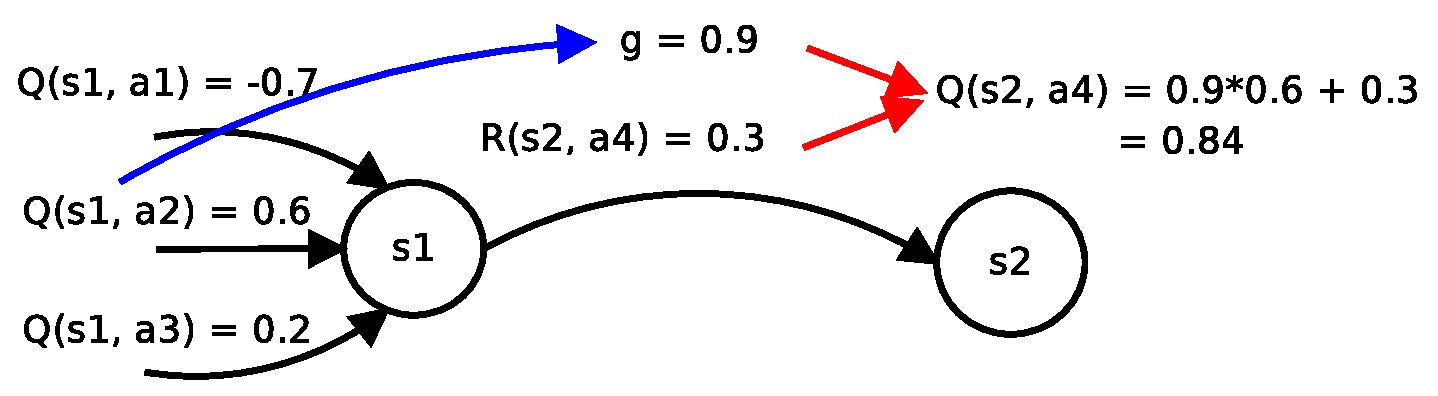
\includegraphics[scale=.3]{../diagrams/q_learning_detail.eps}
\caption{Q value function for $\gamma = 0.9$}
\label{img:q_learning}
\end{figure}

The term $\max_{a(n-1) \in \mathbb{A}} Q_{n-1}(s(n-1), a(n-1)$ is responsible
for convergence into optional strategy independly on action selection
Another point of view is SARSA algorithm \cite{bib:sarsa}

\begin{align}
Q_{n}(s(n),a(n)) &= \nonumber \\
 (1-&\alpha)Q_{n-1}(s(n),a(n)) + \nonumber  \\
&\alpha(R(s(n),a(n)) + \gamma Q_{n-1}(s(n-1), a(n-1)))
\label{eq:sarsa}
\end{align}

where $\alpha \in (0, 1)$, and $Q_{n}(s(n),a(n))$ set on
mean value and depends on action's selection strategy.

\section{Solution design}

For small state spaces can be $Q_{n}(s(n),a(n))$ stored as table.
In huge spaces, or continuous spaces it is impossible, from two main reasons
\begin{enumerate}
  \item huge memory requirements
  \item all state transactions have to be visited
\end{enumerate}

Function can be approximated, using neural networks.
Common feed forward percepton network can't be learned \cite{bib:q_fnn_problem}.
From neural network is required to compute correct $Q_{n-1}(s(n),a(n))$ values,
and learn value in $Q_{n}(s(n),a(n))$. Learning neural network in $Q_{n}(s(n),a(n))$
changes values in all other points $s$ and $a$. One of solution is to define
basis function neural network
\cite{bib:aproximation_01},
\cite{bib:aproximation_02},
\cite{bib:aproximation_03},
\cite{bib:aproximation_04}.
For finite and discrete count of actions can
be for each action defined own $Q$ function.

Few examples of tested basis functions
\begin{align}
    f_j^1(\boldmath{s(n), a(n)}) &= e^{ -\sum\limits_{i=1}^{n_s}{\beta_{aji}(n)(s_i(n) - \alpha_{aji}(n))^2} }  \\
    f_j^2(\boldmath{s(n), a(n)}) &= \frac{1}{1 + \sum\limits_{i=1}^{n_s}{\beta_{aji}(n)(s_i(n) - \alpha_{aji}(n))^2}}  \\
    f_j^3(\boldmath{s(n), a(n)}) &= e^{ -\sum\limits_{i=1}^{n_s}{\beta_{aji}(n)\mid s_i(n) - \alpha_{aji}(n) \mid} }
    \label{eq:basis_functions_01}
\end{align}

where \\
$\alpha_{aji}(n) \in \langle -1, 1 \rangle$ is maxima position \\
$\beta_{aji}(n) \in (0, \infty)$ function shape.

First two are plotted on fig. \ref{img:basis_funcions}

\begin{figure}[]
\center
\includegraphics[scale=.3]{../pictures/gaussian_1D.png}
\caption{Basis function for one dimension}
\label{img:basis_funcions}
\end{figure}

For symetrical states transactions we can write more simple form

\begin{align}
f_j^1(\boldmath{s(n), a(n)}) &= e^{ -\beta_{aj} \sum\limits_{i=1}^{n_s}{(s_i(n) - \alpha_{aji})^2} }  \\
f_j^2(\boldmath{s(n), a(n)}) &= \frac{1}{1 + {\beta_{aj} \sum\limits_{i=1}^{n_s}(s_i(n) - \alpha_{aji})^2}}  \\
f_j^3(\boldmath{(n)s, a(n)}) &= e^{ -\beta_{aj} \sum\limits_{i=1}^{n_s}{\mid s_i(n) - \alpha_{aji}(n) \mid} }
\label{eq:basis_functions}
\end{align}

Approximate Q-value function can be written as linear combination of $l$
basis functions

\begin{align}
Q^x(s(n), a(n)) = \sum\limits_{j=1}^{l} w(n)_j^x f_j^x(\boldmath{s(n), a(n)})
\label{eq:knn_y_update}
\end{align}

where $w(n)_j^x$ are weights.

These functions have independent parameters, and approximate independent area
of state space. Parameters can be learned separately.



\subsection{Hybrid basis functions}

In Q function can be spotted two basic shapes \ref{img:peak_hill_funcion} - peaks,
and hills. For peaks are reponsible negative $R(s(n), a(n))$ values and for hills
positive $R(s(n), a(n))$ values.

\begin{figure}[]
\center
\includegraphics[scale=.3]{../pictures/peak_hill_function.png}
\caption{Q value function example}
\label{img:peak_hill_funcion}
\end{figure}

We can combine two basic ideas an define new basis function, combining
Gaussian curve with some sharp function

\begin{align}
P_i(s(n), a(n)) &=
\left\{
	\begin{array}{ll}
		r_{ai}  & if \ s(n) = \alpha^1_i \\
		0 & inak
	\end{array}
\right. \\
  H_j(s(n), a(n)) &= w_{aj} e^{ -\beta_{aj} \sum\limits_{i=1}^{n_s}{(s_i(n) - \alpha^2_{aji})^2 }} \\
  Q(s(n), a(n)) &= \sum\limits_{i=1}^{I} P_i(s(n),a(n)) + \sum\limits_{j=1}^{J} H_j(s(n), a(n))
  \label{eq:peak_hill}
\end{align}

where \\
$\alpha^1_j$ are states where $H_j(s(n))$ have non zero values \\
$\alpha^2_j$ are states where $f_j(\boldmath{s(n), a(n)})$ have maximum \\
$r_{ai}$ is negative reward value $R(s(n), a(n))$ \\
$w_{aj}$ is weight \\
$\beta_{aj}$ is shape of Gaussian part, and $\beta > 0$ \\
$I$ a $J$ are numbers of functions \\

Names $P$ a $H$ represent peak and hills.

\section{Experiment results}

For approximation hundreds of experiments were done and statistically computed error values.
Goal is to navigate robot in 2 dimensional space into target. There were 8 actions of movement, which
changes state as $s(n) = s(n-1) + a(n)dt$.
Where set of actions


\begin{align}
\mathbb{A} = [& \nonumber \\
&[0, 1], [0, -1] \nonumber  \\
&[1,  0], [-1, 0], \nonumber \\
&[1, -1], [1, 1], \nonumber \\
&[-1, -1], [-1, 1] \nonumber  \\
					]& \nonumber
\end{align}


There was 64x64 discrete positions - optional
solution can be computed, and used for approximation quality comparsion.
In environment only is one positive reward and few zero rewards, example
of one of four testing environments on fig \ref{img:experiment_reward_function}.

\begin{figure}[!htb]
\centering
\includegraphics[scale=.3]{../../results_q_learning/map_2/reward_value_surface.png}
\caption{Reward function R(s(n), a(n)), map 2}
\label{img:experiment_reward_function}
\end{figure}


For approximation these functions has been tested

\begin{enumerate}
\item sparse table
\item Gauss curve $f_j^1(\boldmath{s(n), a(n)})$, equation \ref{eq:basis_functions}
\item Gauss curve $f_j^1(\boldmath{s(n), a(n)})$ combined with sparse table
\item Kohonen neural network modification siete $f_j^2(\boldmath{s(n), a(n)})$
\item Kohonen neural network modification siete $f_j^2(\boldmath{s(n), a(n)})$ combined with sparse table
\item Gauss curve combined with adaptive table (peak and hill), equation \ref{eq:peak_hill}
\end{enumerate}

Agents trajectory for optional solution can be seen on fig \ref{img:experiment_ref_path}.

\begin{figure}[!htb]
\centering
\includegraphics[scale=.3]{../../results_q_learning/map_2/function_type_0/iterations_10/agents_path_surface.png}
\caption{Agents path, optional solution}
\label{img:experiment_ref_path}
\end{figure}



Summary error results compraing with optional solution for 20 trials runs, in all four envinments are on figures
\ref{img:experiment_average_0},
\ref{img:experiment_average_1},
\ref{img:experiment_average_2},
\ref{img:experiment_average_3}.


\begin{figure}[!htb]
\centering
\includegraphics[scale=.3]{../../results_q_learning/map_0/trials_average_results.png}
\caption{Summary results for map (environment) 0}
\label{img:experiment_average_0}
\end{figure}

\begin{figure}[!htb]
\centering
\includegraphics[scale=.3]{../../results_q_learning/map_1/trials_average_results.png}
\caption{Summary results for map (environment) 1}
\label{img:experiment_average_1}
\end{figure}

\begin{figure}[!htb]
\centering
\includegraphics[scale=.3]{../../results_q_learning/map_2/trials_average_results.png}
\caption{Summary results for map (environment) 2}
\label{img:experiment_average_2}
\end{figure}

\begin{figure}[!htb]
\centering
\includegraphics[scale=.3]{../../results_q_learning/map_3/trials_average_results.png}
\caption{Summary results for map (environment) 3}
\label{img:experiment_average_3}
\end{figure}

And trajectories for three best results
\ref{img:experiment_gauss_path},
\ref{img:experiment_gauss_sparse_table_path},
\ref{img:experiment_gauss_adaptive_table_path}




\begin{figure}[!htb]
\centering
\includegraphics[scale=.3]{../../results_q_learning/map_2/function_type_2/iterations_10/agents_path_surface.png}
\caption{Agents path using Gaussian curve}
\label{img:experiment_gauss_path}
\end{figure}


\begin{figure}[!htb]
\centering
\includegraphics[scale=.3]{../../results_q_learning/map_2/function_type_3/iterations_10/agents_path_surface.png}
\caption{Agents path using Gaussian curve combined with sparse table}
\label{img:experiment_gauss_sparse_table_path}
\end{figure}


\begin{figure}[!htb]
\centering
\includegraphics[scale=.3]{../../results_q_learning/map_2/function_type_6/iterations_10/agents_path_surface.png}
\caption{Agents path using Gaussian curve combined with adaptive table}
\label{img:experiment_gauss_adaptive_table_path}
\end{figure}



\newpage
\section{Conclusions}

From tested function, minimal error occures Gauss curve, Gauss curve combined with sparse table,
and Gauss curve combined with adaptive table (peak and hill function). As we can seen, only
acceptalbe agents trajectory results are for Gauss curve combined with adaptive table.
All experiments results can be visited on \cite{bib:q_learning_git} (more than 10000 results files),
with full access to source codes for further research.

% The following two commands are all you need in the
% initial runs of your .tex file to
% produce the bibliography for the citations in your paper.
\bibliographystyle{abbrv}
{
\litfont
\bibliography{acmbulletin}  % acmbulletin.bib is the name of the Bibliography in this case
}
% You must have a proper ".bib" file
%  and remember to run:
% latex bibtex latex latex
% to resolve all references
%
% ACM needs 'a single self-contained file'!
%
%APPENDICES are optional

\begin{thebibliography}{99}                                \label{literatura}


\bibitem{bib:reinforcement_leraning_01}
Peter Dayan, Christopher J.C.H. Watkins,
Reinforcement Learning
\url{http://www.gatsby.ucl.ac.uk/~dayan/papers/dw01.pdf}


\bibitem{bib:reinforcement_leraning_02}
Daniel Dewey, Oxford Martin Programme on the Impacts of Future Technology,
Future of Humanity Institute :
Reinforcement Learning and the Reward Engineering Principle
\url{http://www.danieldewey.net/reward-engineering-principle.pdf}



\bibitem{bib:markov_01} Markovove rozhodovacie procesy, stručne :
Pieter Abbeel  UC Berkeley EECS : Markov Decision Processes and Exact Solution Methods
\url{http://www.cs.berkeley.edu/~pabbeel/cs287-fa12/slides/mdps-exact-methods.pdf}

\bibitem{bib:markov_02} Martin L. Puterman : Markov Decision Processes: Discrete Stochastic Dynamic Programming
, isbn 9781118625873, rok 2014, \url{https://books.google.sk/books?id=VvBjBAAAQBAJ}


\bibitem{bib:q_learning_watkins}
CHRISTOPHER  J.C.H. WATKINS, PETER DAYAN : Technical Note Q-Learning,
Machine Learning,  8,279-292 (1992)
\url{http://www.gatsby.ucl.ac.uk/~dayan/papers/cjch.pdf}

\bibitem{bib:q_tutorial_01} Q-learning 1
\url{https://www-s.acm.illinois.edu/sigart/docs/QLearning.pdf}

\bibitem{bib:q_tutorial_02} Q-learning 2
\url{http://mnemstudio.org/path-finding-q-learning-tutorial.htm}


\bibitem{bib:q_proof_01} Francisco S. Melo
Institute for Systems and Robotics,
Instituto Superior Técnico,
Lisboa, PORTUGAL : Convergence of Q-learning:  a simple proof
\url{http://users.isr.ist.utl.pt/~mtjspaan/readingGroup/ProofQlearning.pdf}

\bibitem{bib:q_proof_02} Eyal Even-Dar, Yishay Mansour :
Convergence of optimistic and incremental Q-learning,
\url{http://web.cs.iastate.edu/~honavar/rl-optimistic.pdf}


\bibitem{bib:q_proof_03}
Carden, Stephen, "Convergence of a Reinforcement Learning Algorithm in Continuous Domains" (2014).
All Dissertations. Paper 1325.
\url{http://tigerprints.clemson.edu/cgi/viewcontent.cgi?article=2326&context=all_dissertations}

\bibitem{bib:q_proof_04} Francisco S. Melo and M. Isabel Ribeiro,
Convergence of Q-learning with linear function approximation,
Proceedings of the European Control Conference 2007 Kos, Greece, July 2-5, 2007,
\url{http://gaips.inesc-id.pt/~fmelo/pub/melo07ecc.pdf}

\bibitem{bib:sarsa} Karan M. Gupta Department of Computer Science Texas TechUniversity Lubbock, TX 79409-3104 :
Performance Comparison of Sarsa($\lambda$) and Watkin’s Q($\lambda$) Algorithms,
\url{http://www.karanmg.net/Computers/reinforcementLearning/finalProject/KaranComparisonOfSarsaWatkins.pdf}


\bibitem{bib:aproximation_01} Francisco S. Melo, Sean P. Meyn, M. Isabel Ribeiro
An Analysis of Reinforcement Learning with Function Approximation,
Appearing in Proceedings of the 25th International Conference on Machine Learning, Helsinki, Finland, 2008
\url{http://www.machinelearning.org/archive/icml2008/papers/652.pdf}

\bibitem{bib:aproximation_02} David Silver : Lecture 6: Value Function Approximation
\url{http://www0.cs.ucl.ac.uk/staff/d.silver/web/Teaching_files/FA.pdf}

\bibitem{bib:aproximation_03} Francisco S. Melo M. Isabel Ribeiro : Q-learning with linear function approximation
\url{http://gaips.inesc-id.pt/~fmelo/pub/melo07tr-b.pdf}

\bibitem{bib:aproximation_04} Marina Irodova and Robert H. Sloan : Reinforcement Learning and Function Approximation,
2005,  American  Association  for  Artificial  Intelli-gence (www.aaai.org)
\url{http://citeseerx.ist.psu.edu/viewdoc/download?doi=10.1.1.81.7833&rep=rep1&type=pdf}


\bibitem{bib:q_fnn_problem}
Mae L. Seto Springer Science \& Business Media, 9. 12. 2012,
Marine Robot Autonomy, ISBN	1461456592, chap 7.3.3.2



\bibitem{bib:mototko_video} video robota Motoko Aftermath
Michal Chovanec, youtube
\url{https://www.youtube.com/watch?v=8sskJN_zuko}

\bibitem{bib:q_learning_git} Michal Chovanec, Q-learning zdrojové súbory \url{https://github.com/michalnand/q_learning}

\bibitem{bib:motoko_git} Michal Chovanec, Motoko robot zdrojové súbory \url{https://github.com/michalnand/motoko_after_math_linefollower}


\end{thebibliography}








\balancecolumns
% That's all folks!
\end{document}
